\documentclass[a4paper,twoside,notitlepage,11pt]{article}
\usepackage{graphicx}
\usepackage{hyperref}
\usepackage{amstext}
\usepackage{tabularx}
\usepackage{amssymb}
\usepackage{fancyhdr}
\usepackage{setspace}
\usepackage{fancyvrb}
\usepackage[all]{xy}
\usepackage{stmaryrd}
\usepackage{nccmath}
\usepackage[a4paper,hmargin=50pt,vmargin=75pt]{geometry}
\usepackage[hypcap]{caption}
\usepackage{qtree}
\usepackage{cleveref}
\usepackage[normalem]{ulem}
\usepackage{float}
\usepackage{layouts}
\usepackage{wrapfig}
\usepackage{listings}
\usepackage{color}
\usepackage{mathpartir}
\usepackage{fancyeq}
\usepackage{menukeys}

\newcommand{\paperTitle}{Niceway.to Design Specification}
\newcommand{\from}{\leftarrow}

\pagestyle{empty}
\renewcommand{\headrulewidth}{0.0pt}

\fancypagestyle{plain}{
\fancyhf{}
\fancyhead[LE]{\thepage}
\fancyhead[CE]{\textit{\paperTitle}}
\fancyhead[RE]{Craig Knott}
\fancyhead[LO]{Craig Knott}
\fancyhead[CO]{\textit{\paperTitle}}
\fancyhead[RO]{\thepage}
}

\begin{document}

\begin{center}
 \ \\[4cm]
 {\LARGE \textbf{\paperTitle} \\ [0.2cm]}
   \textbf{Craig Knott} \\
    \textbf{Version 1.0}\\
	 \textbf{\today}
\end{center}

 \tableofcontents
  \newpage
   \pagestyle{plain}
 
 \section{Requirements}
 \subsection{Functional Requirements}
 \begin{enumerate}
 \item[1.] The user should be able to search by geographic region and discover submitted plans for that region.
 \item[2.] The user should be able to contribute routes.
 	\begin{enumerate}
 	\item[2.1.] Only the creating user should be able to modify these routes
 	\item[2.2.] The user should be able to decide on the visibility of this route (private or public)
 	\end{enumerate}
 \item[3.] The user should be able to interact socially with the route, including:
 	\begin{enumerate}
 	\item[3.1.] Comment on routes
 	\item[3.2.] Recommend alternative routes
 	\item[3.3.] Share routes to external social media websites
 	\end{enumerate}
 \item[4.] Users should be able to create accounts and specify for example, name, age, email and location 
 \item[5.] The should be administrative users who have extra functionality available, including:
	 \begin{enumerate}
 		\item[5.1.] Manage users
 		\begin{enumerate}
 			\item[5.1.1.] Delete users
 			\item[5.1.2.] Update users
 			\item[5.1.3.] Create users
 		\end{enumerate}
 		\item[5.2.] Manage routes
 		\begin{enumerate}
 			\item[5.2.1.] Delete routes
 			\item[5.2.2.] Update routes
 		\end{enumerate}
 		\item[5.3.] Moderate comments
 		\begin{enumerate}
 			\item[5.3.1.] Delete comments
			\item[5.3.2.] Update comments
 		\end{enumerate}
 		\item[5.4.] Make announcements
 	\end{enumerate}
 \item[6.] Users should be able to export their journeys
 \item[7.] Users should be able to fork other user's public journeys (make a copy), and edit as they wish
 \item[8.] There should be a journey editor component which allows the user's to create and specify their route
 \item[9.] There should be a journey viewer component which visualizes a user's route
 \end{enumerate}
 
 
 \subsection{Non-Functional Requirements}
 TBD
 
 
 \section{Annotated Designs}
 \subsection{Design One}
  \subsection{Design Two}
   \subsection{Design Three}
 
{ \color{red}
 Main pages of the app-
 \begin{enumerate}
  \item Landing Page\\
  Journey viewers fills the majority of the page, search functionality above allowing users to find interesting journeys by geographic location
  \item Account Creation Page\\
  Allow users to create accounts, potentially through Google, twitter and facebook?
  \item Login Page\\
  Allow existing users to log in
  \item Account Details Page\\
  View and update account details, list their journeys, list their comments and updates of comments made on their journeys (and forks?)
  \item Adminstration Page\\
  View real time and historic data for load levels, active users, journey creations, sessions, etc.
 \item Route Creation Page
 \item Route Discovery Page\\
 Members only page similar to landing page but with social commentary
 \end{enumerate}
 

 }
 \subsection{User Flow Diagram}
 
 \begin{figure}[!ht]
 \begin{center}
 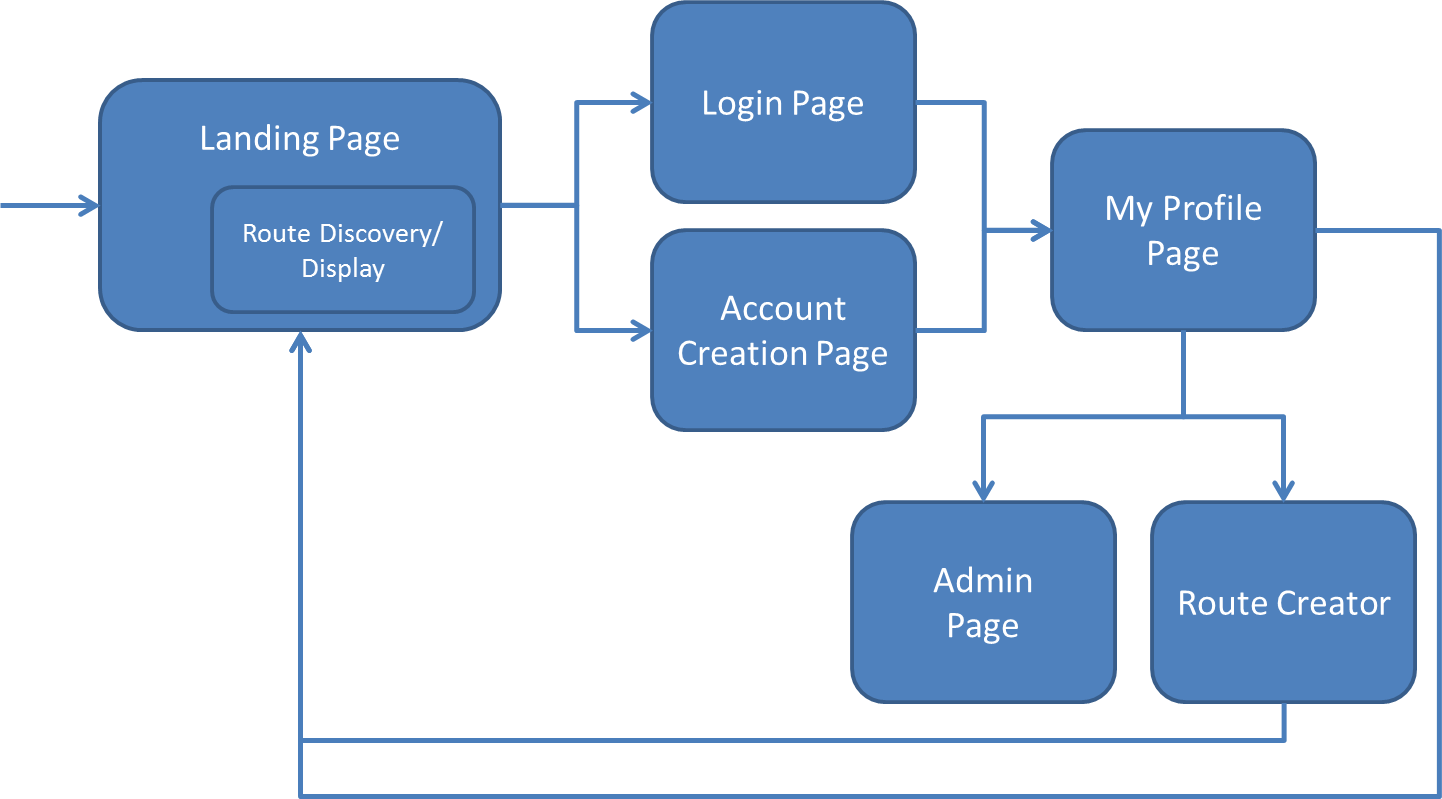
\includegraphics[width=0.7\textwidth]{images/flow.png}
 \end{center}
 \vspace{-6mm}
 \end{figure}
 
 
\section{Market Research}
\subsection{Analysis Of Similar Applications}
\paragraph{Google Maps}
\paragraph{City Mapper}
\paragraph{Apple Maps}
\subsection{Web Applications VS Native Mobile Applications}

\paragraph{Web Applications}\ \\
Web applications are easy to write and don't require knowledge of a specialized language, as the front end is in HTML, CSS and JavaScript, and the backend can be whichever language the programmer is most comfortable with. As they are hosted on the internet, there is no need for the user to download them, which is something that sometimes puts people off from using a service, this also means that if the application is updated, they don't need to install any updates, and can get straight back to using the application. Web applications don't require any approval before being distributed, as they don't need to be put on an app store, and as soon as they are up, they are available to everyone, regardless of their device (unlike mobile apps, which generally target one specific operating system). However, not being on an app store means it's more difficult to discover the application; native applications, are all visible within the market place, which is a lot smaller than the entirety of the world wide web. Another negative of web applications is that they require an internet connection to access (as they are web based), and they cannot fully utilise the native technology of the device they are on (unlike mobile apps which can access all the hardware of the phone they are on). However, web application advertisements are generally less intrusive than mobile ones, so running the application for free is much easier.

\paragraph{Native Mobile Applications}\ \\
Native mobile applications are good because they allow for greater exposure, as they have to be distributed through the app market place. This means there is a centralised place that your application will always be advertised on (although there is a negative that the application has to be submitted to the app store, and may require modifications to get it accepted, which could waste valuable time). This allows for multiple pricing models, a payment for downloading the app (which is less appealing for the user), or for free, with adverts (better, but sometimes the adverts can be very intrusive), or a free version, with the option to upgrade to remove adverts (best of both worlds). Native mobile applications can also be used offline, as they (generally) download all the content onto the user's phone, so it can be accessed regardless of internet connection (this however, is not really applicable to this project, because of the nature of it). This does mean, however, that the app needs to be downloaded (which is generally accepted nowadays, but could also lead to the app being ignored if the user, for instance, doesn't have enough space to download it), and any further updates to the application would need to be downloaded as well. While the application can utilise all the phone's native technology, it is only available for the platform that it was designed for (unless a tool to convert it is used, but this generally produces poor quality products). 
 
 
\end{document}